\documentclass[sigconf]{acmart}

\settopmatter{printacmref=false}
\renewcommand\footnotetextcopyrightpermission[1]{}
\pagestyle{plain}

\usepackage{dirtytalk}
\usepackage{graphicx}
\graphicspath{ {images/} }


\begin{document}
\title{Big Data and Transportation}

\author{Syam Sundar Herle}
\orcid{HID219}
\affiliation{%
  \institution{Indiana University}
  \streetaddress{711 N Park Ave}
  \city{Bloomington} 
  \state{Indiana} 
  \postcode{47408}
}
\email{syampara@iu.edu}

\begin{abstract}

With the rise of population in cities, commutation by road or rail have become hard for people. Transit plays major role in public and private day to day life, but there are limited number of system to address the transportation issues. On other hand Big Data have proved to be more effective and helpful in most of the sectors and business. Big data is all about realizing full potential of large data set by acquiring, storing and managing by advanced technologies and optimizing techniques. With the help of new era of technologies like internet, social media, traffic camera,feeds and smart-phones one can have access to more real-time data which contains abundant of information, which can be used in transportation sector. We can use advance Big Data technologies like Spark on those real-time data set to address transportation issues to build next level Intelligent Transportation Systems (ITS). 

\end{abstract}

\keywords{i523, HID219, Big Data, Intelligent Transportation Systems}

\maketitle

\section{Introduction}

In modern era, technologies plays a major role in our day to day life changing the way of our interaction and livelihood. Smart-phones have become unsaid finger for our hand and internet have pushed communication to next level. The revolution made by technologies and internet have resulted in collection of large real-time data. Real-time data coming from transport camera's, mobile devices, social media's and other sources need to be dealt to provide easy decision making system for commuter in order to set a effective transportation system. According to \cite{bdtrans} \say{the volume and speed at which data are generated, processed and stored is unprecedented}. Said that, Big data is all about realizing full potential and revealing hidden patterns of large data set by acquiring, storing and managing by advanced technologies and optimizing techniques. 

The overwhelming real-time data collected from mobile devices and social media like Facebook, Twitter while travelling contains not only the location based information of the users but also the nature of traffic in hidden manner. These real-time data collected from social media applications and traffic camera can be used to predict the nature of road ahead, optimized route, traffic forecasting and predict them before they occur for the public by Intelligent Transportation system(ITS)\cite{its}. The nature of the data are in diverse manner ranging from structured to unstructured, as these are in real-time the consumed data size would be in terabytes. Because of the huge amount of big data and its nature there is a urgent need of addressing the issues like storing, managing and analyzing which are beyond the capacity of the traditional tools which are used for analysis.


\section{what is Big Data}

As defined earlier, Big data is all about realizing full potential and revealing hidden patterns of large data set by acquiring, storing and managing by advanced technologies and optimizing techniques. According to \cite{bigdata} Big Data has also been defined as by the four V's:

\subsection{Volume}

The mass of amount of the data, which indicates to the data in low level. Lot's of data collected from social media platform are variety and huge amount in nature, which consists of structured and unstructured. Looking up the unstructured data will be futile and we cannot mine any useful information from the raw unstructured data. Advance technologies like Hadoop, Map Reduce \cite{mapreduce,hadoop} needs to employed to manage storage and mine the unstructured data.

\subsection{Velocity}

This can be defined by the rate of pace at which the data are accumulated. In some real-time applications like Internet of Things (IoT) related to health care systems and transportation systems there is a need to evaluate real-time data. Instead of writing high streams of data we need to store it directly to memory to evaluate them. 
\subsection{Variety}

Usually variety can be defined as mixture, when coming to data there will be structured, semi-structured and unstructured. Data like text, audio and video will be unstructured in nature, we need to process to make the unstructured data meaningful and we need to tag the data in same format of the structured data and apply the same techniques which are applied on the structured data. In the case of real time data some of the structured data may change to unstructured or semi-structured without notice.

\subsection{Value}

All data has hidden value, which must be revealed by employing range of technique's depending on the nature of value of the data. The technique's employed usually vary from the quantitative and investigative to discover the real value of the data ranging from expression of the consumers to financial status of the consumers.


Big Data analytic techniques are applied on large data to generate knowledge and reveal hidden patterns which can be harnessed to make useful in customer point of view. Now a days, Big Data analytic are used in many areas like DNA analysis, machine learning, deep learning, robotics and data classification. Usually the Big Data process can be visualized as in the Figure ~\ref{fig:BD}.


\begin{figure}
\centering
\fbox{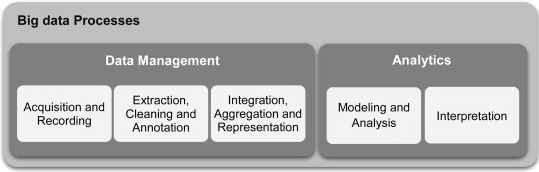
\includegraphics[width=\linewidth]{Capture1}}
\caption{Big Data Process \cite{bigdata}.}
\label{fig:BD}
\end{figure}

 The Big Data process can be broken down to two major component, Data Management and Data Analytic. In Data management segment the large set of data are acquired and recorder as first step, later the data are extracted from the storage or recorded devices and cleansed and annotated to meta file in the case of the unstructured data like video, text and audio. After cleaning and annotation the data are aggregated and presented in order to extract useful information. The unstructured data aggregated and integrated in this step to represent it as a structured data. In the next step Big Data Analytic are employed on the aggregated data, the first step of the analytic is the creation of model to apply on the aggregated data to perform analysis to reveal hidden value and pattern. In the next step visualization of the hidden pattern in the data is done and then the pattern are interpreted to make useful decision making to make a effective system for the consumer needs.
 
 \section{Overview of Big Data Analytic}
 In the following subsection we will look into the available Big Data analytic for structured and unstructured data.
 
 \subsection{Text Analytic}
 
 Extracting information from text data accumulated from social media, online questionnaire, survey and online feeds is known as Text Analytic. A number of analysis and model involved in text analytic like machine learning algorithm, natural language processing and linguistics. The following are the mining techniques are applied in the section of text analytic:
 
 
\subsubsection{Information Extraction}

These techniques extract structured meaning from the unstructured data. These techniques work in two sub task which are Entity Recognition (ER) \cite{bigdata} and Relation Extraction (RE) \cite{bigdata}.

\subsubsection{Text Summarizing}

As the name suggests these techniques create key points of single or multiple document in a succinct way. This analytic technique are employed in two ways, \say{Extractive Approach}\cite{bigdata} and \say{Abstractive approach} \cite{bigdata}. In the \say{Extractive Approach} summary is created from original statements and these summaries are subset of the original document by determining the salient points and putting them together. While the \say{Abstractive Approach} does the extraction of the semantic information from the text by employing Natural Language Processing techniques.

\subsubsection{Questionnaire}

These techniques provides answers to the questions, some of the edge of day applications are Apple Siri and Google Home \cite{bigdata}. Machine learning algorithm like deep learning and speech recognition and artificial intelligence are employed in the Questionnaire technique.

\subsubsection{Opinion Mining}

Opinion Mining are sentiment analysis, where Natural Language Processing and machine learning are employed to mine and classify emotion of the consumer in related to product or governance of a government. Usually text generated from online review portal or social media application like Twitter, Facebook are used to do sentiment analysis.


\subsection{Audio Analytic}

Audio Analytic are employed on the structured and unstructured audio data to extract information, which are used to evaluate consumer needs and evaluating turn over of a company product and to evaluate agent performances. Most of the call centers use the Interactive Voice Response (IVR) \cite{ivr} platforms to identify and handle frustrated customers. In health-care sector, audio analytic are employed to evaluate patients with certain medical condition like depression, schizophrenia \cite{bigdata}. Audio Analytic are done by two ways large-vocabulary continuous speech recognition (LVCSR) \cite{bigdata} and phonetic based approach \cite{bigdata}.

\subsection{Video Analytic}

Video Analytic employs a variety of process like monitoring, analyze and extract useful information from video data. Growth of CCTV usage and video sharing portal usage have increased the need for effective and efficient application and technologies to store and clean and analyze the video data. Text Analytic and Audio Analytic can be used to index the video data for the easy retrieval. Extracted information from the video data can be useful in relating consumer needs based on demographic locations and to derive decisions of the product endorsement in retail sector. The system architecture for video analytic can be done in two ways, Server-based architecture and Edge based architecture.

\subsection{Social Media Analytic}

Analysis of the structured and unstructured data from social media is known as social media analytic. Social media can be categorized as social network (Twitter, Facebook), micro-blog (Reddit) and video sharing (YouTube). The two sources of social media analytic are content shared by users (videos,text and audio) and communication between entity and networks (people and organization). Social Media analytic can be categorized as:

\subsubsection{Content based analytic \cite{bigdata}}
    
The content based analytic are the analyze done on the content posted by people or participant of the social media like Facebook, Twitter. These content based data are large set of unstructured data such as videos, text and audio files. The Text Analytic, Audio Analytic and Video Analytic are usually employed on these type of data-sets to mine useful information.
    
\subsubsection{Structure based analytic \cite{bigdata}}

Structure based analytic usually related to the extraction of relation among the entities or participant of the social media. Social network are modelled through edge and nodes to represent the entities and the relationship among the entities.



\subsection{Predictive Analytic}

Prediction of future outcome using data is known as Predictive Analytic. The data for these type of analytic can be categorized as, real-time and historical data. Primarily predictive analytic is based on statistical models applied on data to predict the outcome of future or predict the relationship among the data. When predicting the outcome of future techniques such as moving average are employed on the historical data. On the real-time data techniques like linear regression are applied to predict the relationship among the data. Predictive analytic are applied in two ways, statistical model applied on sample population of the data which is further applied to full scale data. The other way is usage of computational techniques applied on full scale big data to do the predictive analytic.  
 
\section{Transportation}

Transportation is a means of transporting goods and people between different location, it is a vital element of modern society. Since the earliest days of the industrial revolution, transportation has facilitated economic development by moving materials, resource, products and people \cite{trans}. Transportation around the world have some common problems, which causes disruption of not only road traffic but also it has effects on the economic and as well as ecosystem of country.

Common problems in transportation,

\begin{itemize}
\item Road traffic
\item Environmental Pollution
\item Accidents
\item Inability of forecasting traffic
\item Road Maintenance
\item Road Construction/Maintenance 
\end{itemize}

Creation of a transportation system need to address the above problems, when implementing a transportation, government needs to address to avoid the future traffic congestion in case of road maintenance of road construction. Road accidents costs more than life cost, like insurance, rehabilitation cost, property damage cost and so on. Pollution impact also need to be addressed when designing and implementing a effective transport system, if CO2 emission is unchecked it may lead to health related problem and global warming.

Apart from mentioned problem's, creation of a transport system also needs to address some to the issues related to city planning also, the problems can be categorized in the following subsections,

\begin{enumerate}
\item City Plan 

The plan of the city is very crucial, specifically in cities as the traffic congestion as to be addressed. 

\item Police and Law Enforcement 

Consideration of traffic law is also very important, speed limits are also important to taken into consideration.

\item Event Gathering 

During specific social event gathering, road block and alternative route have to be taken into consideration.

\end{enumerate}

The above issues highlights specifically the situation of the road congestion and road traffic, so the government or transport system planning body should take necessary considerations in the above stated problems by investing sufficient time and money for installing the surveillance and tools. 


\section{Existing Transportation system using Big Data Analytic}

Different countries have employed different big data technologies for their transportation systems project to ease the traffic and make an efficient and social impact transportation. Some of the projects are as follows:


\subsection{Public Transit System, Ireland}

The country of Ireland came up with an Public Transit System project \cite{bdlt}. IBM big data analytic helped them to come up with an intelligent public transportation system and ease the traffic congestion. The data sources of this were GPS data, speed data, Stop data and fare data collected from Bus System of Ireland and real-time video stream data from CCTV footage and  Ireland road weather condition and road work data as an CSV formatted files. real-time road sensor data were also used to build Public Transit System. Advanced analytic concepts were applied on the data to identify traffic congested areas and alternative in the case of road maintenance. 

\subsection{Real-time vehicle monitoring system, India}

The government of India came up with Real-Time vehicle monitoring program \cite{bdlt} using advanced analytic tools to ease operational complexion in logistic and transportation. The data collected from vehicle sensors and GPS devices are used to study about the vehicles fuel status, speed, acceleration and location. All the unstructured data are stored in HDFS system and monitored on consistent time interval to improve logistic productivity.

\subsection{Air travel customer analysis system, United Kingdom}

Air travel customer analysis system \cite{bdlt} was developed by United Kingdom to understand the needs of the clients of the aviation industries. The data collected from social media, call center and Smart-phone device were used to do Predictive Analytic and Social Media Analytic to identify the customer needs and problems to improve the standard of service provided in the Aviation industry of United Kingdom.

\subsection{Real-time Intelligent Transportation system, Sweden}

Sweden created a project based on IBM InfoSphere \cite{bdlt} to improve the transportation network in their city of Stockholm. For this project the system collected data from taxi vehicle GPS along with link related to location information to create a Real-Intelligent Transportation system to predict future traffic condition and shortest-route to destination for public and law enforcement agencies


\section{conclusion}

We came across what is big data and type of big data analytic employed based on different nature of data accumulated from different data sources and some of the existing transportation system employed in different countries using Big Data Analytic. Even-though there are good transportation system employed using Big Data Analytic, with the current advancement in integration and penetration of machine learning, artificial intelligence and Big Data Analytic tools like Apache Hadoop and Spark, an edge of the day Intelligent Transportation System can be developed to use in areas like congestion management, traffic routing and scheduling.

\section*{Acknowledgements}

The author would like to thank Dr. Gregor von Laszewski and his teaching assistants for providing helpful feedback.


\bibliographystyle{ACM-Reference-Format}
\bibliography{report}

\end{document}
